\chapter{PEOPLE GAZETTEER}
\label{chapter:people gazetteer}

 %Define ppl gazetteer in chapter 1 and why is it required.
People Gazetteer as defined in Chapter 1 consists of tuples of person names along with list of documents in which they occur and their corresponding topics. This chapter describes the 2-step process of construction of the People Gazetteer by
a) Extraction of person names from the news articles dataset using Named Entity Recognition in  Section~\ref{ner} and
b) Assignment of topics to news articles using LDA topic detection in  Section~\ref{topic detection}.
Output of People gazetteer developed using these steps is presented in Section ~\ref{gaz:result}.

\section{Person Named Entity Recognition (PNER)}
\label{ner}


\subsection{Definition}
NER (Named Entity Recognition) refers to classification of elements in text into pre-defined categories such as the names of persons, organizations, locations, expressions of times, quantities, monetary values, percentages, etc. 
Person Named Entity Recognition (PNER) can be defined as the process of NER that marks up only person names that occur in the text.

PNER is required in this research so as to extract all person name entities occurring in the complete dataset and identify influential person entities among them through development of the People Gazetteer. 
PNER aids in the development of People Gazetteer by first extracting all person names occurring in the dataset followed by reverse linking of a person with the articles in which he/she occurs.

\subsection{Methodology}

The Stanford CRF-NER\footnote{http://nlp.stanford.edu/software/CRF-NER.shtml} is used for PNER in this research. It can perform NER for 3 classes: Person, Organization and Location and is based on linear chain CRF (Conditional Random Field) sequence models. It is trained across several corpora and is fairly robust across multiple domains and even better when compared to some other open source NER systems as illustrated in \cite{rodriquez2012comparison}. According to their results, Stanford NER gave overall the best performance across 2 OCR datasets, and was most effective for PNER when compared with 3 other open source NER systems.


\subsection{PNER Results}

\begin{figure}[h]
  \centering
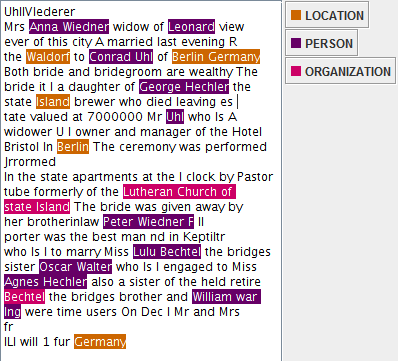
\includegraphics{NER1}
\caption{NER on a sample news article}
\label{figure:sample}
\end{figure} 




NER on a sample news article from the dataset can be seen in Figure ~\ref{figure:sample}.
 Stanford NER recognizes a person's full name as separate names by default which is rectified by combining these multi-term entities into single person entities. Person names tagged with ``PERSON" category are stored while running NER on the dataset.
Whenever a person name occurs in a document, the person entity's name along with the document name is stored to obtain tuples of person names with their document lists.
The Stanford NER takes 25 minutes to run on the complete news dataset of 14020 articles extracting a total of 38426 person entities. The output obtained can be seen in Table ~\ref{table:Table1} which shows the number of person entities with the corresponding number of documents in which they occur.  


\begin{table}[h]
  \begin{center}
\begin{tabular}{|l|l|l|}
    \hline
\textbf{No. of Person Entities} & \textbf{No. of articles} \\ \hline
36616                  & 1               \\ \hline
1123                   & 2               \\	\hline
329                    & 3               \\	\hline
123                    & 4               \\	\hline
87                     & 5               \\	\hline
48                     & 6               \\	\hline
29                     & 7               \\	\hline
19                     & 8               \\	\hline
16                     & 9               \\	\hline
5                      & 10              \\	\hline
4                      & 11              \\	\hline
6                      & 12              \\	\hline
4                      & 14              \\	\hline
3                      & 15              \\	\hline
2                      & 16              \\	\hline
1                      & 17              \\	\hline
1                      & 18              \\	\hline
3                      & 19              \\	\hline
1                      & 20              \\	\hline
1                      & 21              \\	\hline
1                      & 22              \\	\hline
1                      & 23              \\	\hline
1                      & 27              \\	\hline
1                      & 29              \\	\hline
1                      & 31              \\	\hline
1                      & 34              \\	\hline
1                      & 35              \\ 	\hline
\end{tabular}
\end{center}
\caption{Table showing output of PNER on 14020 articles}
\label{table:Table1}
\end{table}



We divide the people entities extracted into following categories so that separate analysis can be done for each category:
\begin{description}
 \item[$\bullet$Marginally Influential]: This category includes all person entities with occurrence in 4 or below news articles. (38189 person entities as calculated from Table 5.1)
\item[$\bullet$Medium Influential]: This category includes all person entities with occurrence between 5 and 15 news articles. (221 person entities) 
\item[$\bullet$Highly Influential] : This category includes all person entities with occurrence in more than 15 news articles. (16 person entities)
\end{description}



\section{Topic Detection}
\label{topic detection}

 Topic models are algorithms for discovering the main topics that occur across a large and otherwise 
unstructured collection of documents and can organize the collection according to the discovered topics.
Here, a topic refers to a set of words which describe what any document is about.
 A topic model examines the set of documents and discovers based on the statistics of the words in each, what the topics might be and what each document's balance of topics is.
Documents are considered as a mixture of topics and each topic a probability distribution over words.
 Topic detection is the process of identifying topics in a document collection using a topic model. A simple example of topic model illustrated by \cite{blei2012probabilistic} can be seen in Figure 5.2.
Topic detection is essential to this research in order to determine the topics of individual news articles that a person entity occurs in so that the person entity can be linked to the documents in which he/she occurs along with their respective topics.

%DOUBT--Whether to mention if: The discovered topics for articles are further used to detect influential persons across multiple articles topics.


\subsection{Topic Detection Model}


\begin{figure}[h]
\centering
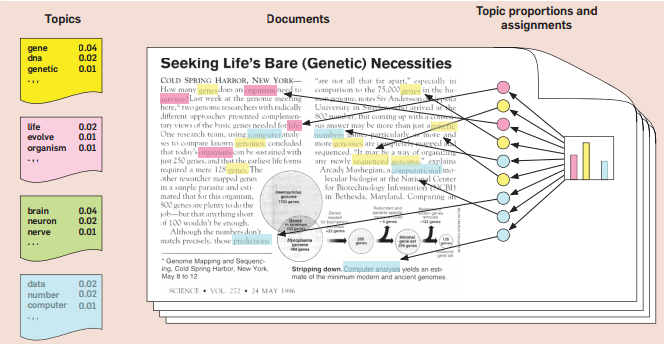
\includegraphics{topicmodel}
\caption{Simple topic modelling approach for a single article\cite{blei2012probabilistic}.}
\end{figure} 

A simple parallel threaded LDA model described in \cite{newman2007distributed}  is used for topic detection in this research.
LDA (Latent Dirichlet Allocation) is a generative probabilistic model in which each document is modeled as a finite mixture over an underlying set of topics and each topic, in turn, is modeled as an infinite mixture over an underlying set of topic probabilities\cite{blei2003latent}. In other words, documents exhibit multiple topics and each topic is a distribution over a fixed vocabulary. 
%The model was developed as an improved version of Probabilistic Latent Semantic Indexing.
Given an input corpus of `D' documents with `K' topics, the LDA learning process consists of calculating `${\Phi}$', 
maximum-likelihood estimate of model parameters. Given this model, we can infer
topic distributions for arbitrary documents.  
However, this simple LDA approach can take several days to run over a large corpora which is why PLDA suits to large datasets such as ours.


The PLDA model uses distributed computation where total dataset is distributed equally among multiple processors. Initialization involves data and parameters distribution to each processor and random assignment of topics so that each processor has its own copy of data, word topic and topic counts. The topic model inferencing then uses simultaneous local Gibbs sampling approach on each processor for a pre-decided number of iterations to reassign topic probabilities, word topic and topic counts. Global update is performed after each pass by using a reduce-scatter operation to get a single set of counts and obtain final topic assignments.
The PLDA model requires user set parameters before inferencing like Number of topics, Number of words in a topic and Dirichlet parameters. 


\subsection{Results}

Parallel LDA model implemented in the Mallet\cite{McCallumMALLET} toolkit is used for topic detection over the complete dataset of 14020 news articles. 
Several topic models are implemented with different parameter settings in order to decide the number of iterations and topics for the final topic model. The different topic models can be evaluated using Perplexity measure calculated through the following formula:
Perplexity= e(-Log Likelihood of held out test test/No. of tokens in held out test set)

Topic Modeling is done for 500 iterations and two parallel samplers, which each look at one half the corpus and combine
statistics after every iteration. It takes 2 hours to run PLDA on the complete dataset.
 For each news article, a set of topics with their probability distribution score for the article is obtained out of which the topic with highest topic probability score is associated with the article.  
We obtain different results from topic detection with following parameters setting:
\begin{enumerate}
 \item Number of topics(k) = 30, Number of iterations = 500
 \item Number of topics(k) = 100, Number of iterations = 500
\end{enumerate}
The set of 30 topics obtained through topic detection on the dataset are illustrated in Figure ~\ref{figure:topicwords}. The most common topic among the news articles highlighted is highlighted as Topic 0 with the words: ``club, line,street,game,total,won,team,time,half, race".


\begin{table}[h]
\centering
\begin{tabular}{@{}lc@{}}
\cmidrule(r){1-1}
\multicolumn{1}{|l|}{Topic ID} & Topic Words \\ \midrule
\multicolumn{1}{|l|}{0} & \begin{tabular}[c]{@{}c@{}}total ii won club score night ran furlough alleys tournament time\\   mile fourth rolled curling scores race national game\end{tabular} \\ \midrule
1 & la lu ot lo tu au tb ta ha tea day al aa ut ar uu wa tt te \\
2 & \begin{tabular}[c]{@{}c@{}}iii lie tin nail tn lit hut ill ii nn thu tu anti thin inn hit lu lo\\   nut\end{tabular} \\
3 & \begin{tabular}[c]{@{}c@{}}line street feet point western easterly northerly feel southerly\\   distance place distant lo fret hue beginning laid early felt\end{tabular} \\
4 & \begin{tabular}[c]{@{}c@{}}opera theatre music company week play stage evening night performance\\   concert mme audience manager season de orchestra house miss\end{tabular} \\
5 & \begin{tabular}[c]{@{}c@{}}great people life man women good country world american part ot ha\\   made la years make long place bad\end{tabular} \\
6 & \begin{tabular}[c]{@{}c@{}}election mr party republican state district vote democratic county senator\\   elected city committee mayor political candidate majority york democrats\end{tabular} \\
7 & \begin{tabular}[c]{@{}c@{}}time ho work tn men city bo lie anti day thin long thu made part ago\\   lot york make\end{tabular} \\
8 & \begin{tabular}[c]{@{}c@{}}st room av sun wife board front lo december rent lot november sunday\\   ht west ar house private si\end{tabular} \\
9 & \begin{tabular}[c]{@{}c@{}}dr book st story books cloth author cure free work york blood\\   illustrated remedy goods medical library health price\end{tabular} \\
10 & \begin{tabular}[c]{@{}c@{}}company york trust bonds city cent railroad mortgage interest wall\\   bond stock street st central january coupon committee jan\end{tabular} \\
11 & \begin{tabular}[c]{@{}c@{}}church dr father funeral school st college sunday year rev catholic\\   pastor services late service held society holy clock\end{tabular} \\
12 & \begin{tabular}[c]{@{}c@{}}horse race class horses won racing years prize record year show ring\\   track mile money jockey trotting trotter ran\end{tabular} \\
13 & \begin{tabular}[c]{@{}c@{}}cent year week pf market total net stock today central st ft lit\\   sales short cotton ohio lot month\end{tabular} \\
14 & \begin{tabular}[c]{@{}c@{}}white water indian black long found thu big dog time ground wild tree\\   killed birds bird day great lake\end{tabular} \\
15 & \begin{tabular}[c]{@{}c@{}}price black silk goods prices ladies worth dress fine white full tea\\   quality style wool made fancy cloth fur\end{tabular} \\
16 & \begin{tabular}[c]{@{}c@{}}street mrs mr avenue wife house miss yesterday years home woman night\\   ago husband found died daughter children mother\end{tabular} \\
17 & \begin{tabular}[c]{@{}c@{}}war american government army chinese japanese china japan foreign\\   united nov emperor states prince minister military french port navy\end{tabular} \\
18 & \begin{tabular}[c]{@{}c@{}}feet north minutes avenue boundary seconds degrees west york minute\\   degree point east south feel city angle county laid\end{tabular} \\
19 & \begin{tabular}[c]{@{}c@{}}man ho men night back wa room left house told bad door found turned place\\   ran lie front morning\end{tabular} \\
20 & \begin{tabular}[c]{@{}c@{}}water feet building boat company car train road fire miles railroad\\   island work line city great river built bridge\end{tabular} \\
21 & \begin{tabular}[c]{@{}c@{}}club game team play football half ball left college back yale played\\   harvard line eleven men match yacht field\end{tabular} \\
22 & ii iii ill lit ll si ti il im vi st iv ft mi li till lull lui oil \\
23 & \begin{tabular}[c]{@{}c@{}}bank money national gold amount notes banks hank business treasury\\   account cent paid bonds note currency company stock estate\end{tabular} \\
24 & \begin{tabular}[c]{@{}c@{}}mr john william york henry charles james club city ii george dec dr\\   thomas smith jr brooklyn van held\end{tabular} \\
25 & \begin{tabular}[c]{@{}c@{}}piano st rooms car york daily chicago city sunday upright parlor\\   furnished broadway hotel av west train brooklyn monthly\end{tabular} \\
26 & \begin{tabular}[c]{@{}c@{}}york daily steamship nov directed letter dec fur orleans al steamer\\   walls letters close australia china japan city london\end{tabular} \\
27 & \begin{tabular}[c]{@{}c@{}}mr court police judge justice case yesterday street district witness\\   jury charge asked attorney trial arrested lawyer told office\end{tabular} \\
28 & \begin{tabular}[c]{@{}c@{}}mr law present made public year state committee president secretary\\   bill report states con tin united number meeting york\end{tabular} \\
29 & \begin{tabular}[c]{@{}c@{}}air ran ur fur ui full tt al tl late mr ant liar art lay told met ti\\   tr\end{tabular} \\ \bottomrule
\end{tabular}
\caption{My caption}
\label{table:topicwords}
\end{table}




The different settings of LDA parameters are experimented further in Chapter ~\ref{chapter:influential people detection} in order to understand their effect on influential people detection.
\section{People Gazetteer Output }
\label{gaz:result}

The list of articles obtained for each person entity after application of PNER and highest scoring topic assigned to each article during Topic Detection are combined to obtain People Gazetteer. In each tuple of the gazetteer, a person entity gets associated with its list of articles where each article is further associated with its corresponding highest scoring topic.

A snapshot of the people gazetteer can be seen in Figure~\ref{figure:gazette} where each person entity is followed by a list consisting of a text Document ID and its corresponding Topic ID. 
\begin{figure}[!h]
\centering
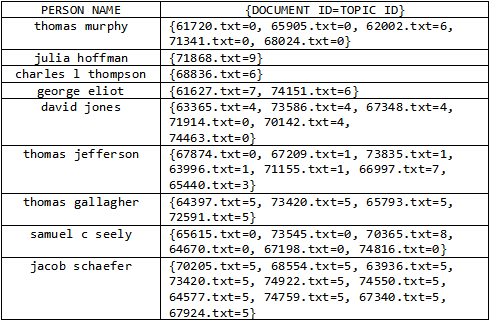
\includegraphics{gazetteer}
\caption{Snapshot of People Gazetteer with Person names, Document list and their corresponding Topic ID}
\label{figure:gazette}
\end{figure} 

%DOUBT: Do the results of people gazetteer need to be presented separately according to each people category: marginal, medium n highly influential?
